% Template LaTeX file for DAFx-14 papers
%
% To generate the correct references using BibTeX, run
%     latex, bibtex, latex, latex
% modified...
% - from DAFx-00 to DAFx-02 by Florian Keiler, 2002-07-08
% - from DAFx-02 to DAFx-03 by Gianpaolo Evangelista
% - from DAFx-05 to DAFx-06 by Vincent Verfaille, 2006-02-05
% - from DAFx-06 to DAFx-07 by Vincent Verfaille, 2007-01-05
%                          and Sylvain Marchand, 2007-01-31
% - from DAFx-07 to DAFx-08 by Henri Penttinen, 2007-12-12
%                          and Jyri Pakarinen 2008-01-28
% - from DAFx-08 to DAFx-09 by Giorgio Prandi, Fabio Antonacci 2008-10-03
% - from DAFx-09 to DAFx-10 by Hannes Pomberger 2010-02-01
% - from DAFx-10 to DAFx-12 by Jez Wells 2011
% - from DAFx-12 to DAFx-14 by Sascha Disch 2013
%
% Template with hyper-references (links) active after conversion to pdf
% (with the distiller) or if compiled with pdflatex.
%
% 20060205: added package 'hypcap' to correct hyperlinks to figures and tables
%                      use of \papertitle and \paperauthorA, etc for same title in PDF and Metadata
%
% 1) Please compile using latex or pdflatex.
% 2) If using pdflatex, you need your figures in a file format other than eps! e.g. png or jpg is working
% 3) Please use "paperftitle" and "pdfauthor" definitions below

%------------------------------------------------------------------------------------------
%  !  !  !  !  !  !  !  !  !  !  !  ! user defined variables  !  !  !  !  !  !  !  !  !  !  !  !  !  !
% Please use these commands to define title and author of the paper:
\def\papertitle{Wavelet Scattering on the Shepard Pitch Spiral}
\def\paperauthorA{Vincent Lostanlen}
\def\paperauthorB{St\'{e}phane Mallat}
\def\paperauthorC{Joseph Fourier}
\def\paperauthorD{Claude Shannon}

\hyphenation{Facto-rization}

%------------------------------------------------------------------------------------------
\documentclass[twoside,a4paper]{article}
\usepackage{dafx_15}
\usepackage{amsmath,amssymb,amsfonts,amsthm}
\usepackage{euscript}
\usepackage[latin1]{inputenc}
\usepackage[T1]{fontenc}
\usepackage{ifpdf}

\usepackage[english]{babel}
\usepackage{caption}
\usepackage{subfig, color}

\setcounter{page}{1}
\ninept

\usepackage{times}
% Saves a lot of ouptut space in PDF... after conversion with the distiller
% Delete if you cannot get PS fonts working on your system.

% pdf-tex settings: detect automatically if run by latex or pdflatex
\newif\ifpdf
\ifx\pdfoutput\relax
\else
   \ifcase\pdfoutput
      \pdffalse
   \else
      \pdftrue
\fi

\ifpdf % compiling with pdflatex
  \usepackage[pdftex,
    pdftitle={\papertitle},
    pdfauthor={\paperauthorA, \paperauthorB, \paperauthorC, \paperauthorD},
    colorlinks=false, % links are activated as colror boxes instead of color text
    bookmarksnumbered, % use section numbers with bookmarks
    pdfstartview=XYZ % start with zoom=100% instead of full screen; especially useful if working with a big screen :-)
  ]{hyperref}
  \pdfcompresslevel=9
  \usepackage[pdftex]{graphicx}
  \usepackage[figure,table]{hypcap}
\else % compiling with latex
  \usepackage[dvips]{epsfig,graphicx}
  \usepackage[dvips,
    colorlinks=false, % no color links
    bookmarksnumbered, % use section numbers with bookmarks
    pdfstartview=XYZ % start with zoom=100% instead of full screen
  ]{hyperref}
  % hyperrefs are active in the pdf file after conversion
  \usepackage[figure,table]{hypcap}
\fi

\title{\papertitle}

%-------------SINGLE-AUTHOR HEADER STARTS (uncomment below if your paper has a single author)-----------------------
\affiliation{
\paperauthorA, \paperauthorB \sthanks{This work is supported by the ERC InvariantClass 320959.}}
{\href{http://di.ens.fr/data/}{Dept. of Computer Science}, \\
\'{E}cole normale sup\'{e}rieure \\
Paris, France\\
{\tt \href{mailto:vincent.lostanlen@ens.fr}{vincent.lostanlen@ens.fr}}
}
%-----------------------------------SINGLE-AUTHOR HEADER ENDS------------------------------------------------------

%---------------TWO-AUTHOR HEADER STARTS (uncomment below if your paper has two authors)-----------------------
%\twoaffiliations{
%\paperauthorA, \sthanks{This work was supported by the XYZ Foundation}}
%{\href{http://dafx14.fau.de}{Fraunhofer IIS,} \\ Friedrich-Alexander University Erlangen\\ Erlangen, Germany\\
%{\tt \href{mailto:dafx14@audiolabs-erlangen.de}{dafx14@audiolabs-erlangen.de}}
%}
%{\paperauthorB, \sthanks{This guy is a very good fellow}}
%{\href{http://music.nuim.ie/}{Dept. of Music,} \\ National University of Ireland\\ Maynooth, Ireland\\
%{\tt \href{mailto:papers@dafx13.nuim.ie}{papers@dafx13.nuim.ie}}
%}
%-------------------------------------TWO-AUTHOR HEADER ENDS------------------------------------------------------

%---------------THREE-AUTHOR HEADER STARTS (uncomment below if your paper has three authors)-----------------------
%\threeaffiliations{
%\paperauthorA, \sthanks{This work was supported by the XYZ Foundation}}
%{\href{http://dafx14.fau.de}{Fraunhofer IIS,} \\ Friedrich-Alexander University Erlangen\\ Erlangen, Germany\\
%{\tt \href{mailto:dafx14@audiolabs-erlangen.de}{dafx14@audiolabs-erlangen.de}}
%}
%{\paperauthorB, \sthanks{This guy is a very good fellow}}
%{\href{http://music.nuim.ie/}{Dept. of Music,} \\ National University of Ireland\\ Maynooth, Ireland\\
%{\tt \href{mailto:papers@dafx13.nuim.ie}{papers@dafx13.nuim.ie}}
%}
%{\paperauthorC,\sthanks{Illustrious contributor}}
%{\href{http://dafx14.fau.de}{Spectral Labs,} \\ Somewhere above the sky\\ {\tt \href{mailto:spectrum@sinus.oids}{mailto:spectrum@sinus.oids}}
%}
%-------------------------------------THREE-AUTHOR HEADER ENDS------------------------------------------------------

%----------------FOUR-AUTHOR HEADER STARTS (uncomment below if your paper has four authors)-----------------------
%\fouraffiliations{
%\paperauthorA, \sthanks{This work was supported by the XYZ Foundation}}
%{\href{http://dafx14.fau.de}{Fraunhofer IIS,} \\ Friedrich-Alexander University Erlangen\\ Erlangen, Germany\\
%{\tt \href{mailto:dafx14@audiolabs-erlangen.de}{dafx14@audiolabs-erlangen.de}}
%}
%{\paperauthorB, \sthanks{This guy is a very good fellow}}
%{\href{http://music.nuim.ie/}{Dept. of Music,} \\ National University of Ireland\\ Maynooth, Ireland\\
%{\tt \href{mailto:papers@dafx13.nuim.ie}{papers@dafx13.nuim.ie}}
%}
%{\paperauthorC,\sthanks{Illustrious contributor}}
%{\href{http://dafx14.fau.de}{Spectral Labs,} \\ Somewhere above the sky\\ {\tt \href{mailto:spectrum@sinus.oids}{mailto:spectrum@sinus.oids}}
%}
%{\paperauthorD,\sthanks{Yes, senior}}
%{\href{http://www.audiolabs-erlangen.com}{Communications Office, Somewhere else,} \\ Centre for Something \\ {\tt \href{mailto:some@where.no }{some@where.no}}
%}
%-------------------------------------FOUR-AUTHOR HEADER ENDS------------------------------------------------------

\begin{document}
% more pdf-tex settings:
\ifpdf % used graphic file format for pdflatex
  \DeclareGraphicsExtensions{.png,.jpg,.pdf}
\else  % used graphic file format for latex
  \DeclareGraphicsExtensions{.eps}
\fi

\maketitle

\begin{abstract}
We present a new reprensetation of sounds that liearizes the dynamics of pitch chroma and pitch height, while remaining stable to deformations in the time-frequency plane. It is an instance of the scattering transform, a generic operator which cascades wavelet convolutions and modulus nonlinearities. It is derived from the Shepard pitch spiral, in that convolutions are performed in time, log-frequency (correlated to pitch chroma) and octave index (correlated to pitch height).
\end{abstract}

\section{Introduction}
Spectrogram-based pattern recognition algorithms, such as sparse coding \cite{Abdallah2004} and Nonnegative Matrix Factorization \cite{Smaragdis2003}, are widespread in audio signal processing.
They are designed to approximate their input by a linear combination of few data-driven templates.
Musical chords, for example, are expected to get decomposed into individual notes.

However, most natural sounds cannot be factorized as amplitude-modulated fixed spectra: notably, continuous changes in pitch (e.g. vibrato, glissando) as well as in spectral envelope (e.g. attack transients, formantic transitions) have a joint time-frequency structure that cannot be matched to a single spectral atom.
Time-varying, under-constrained generalizations have been devised to address this shortcoming \cite{Hennequin2011}, but their high number of parameters prevents their robustness in challenging polyphonic contexts.

Instead of specifying probabilistic priors to help the convergence \cite{Fuentes2013}, we aim to design a template-free, nonlinear, mid-level representation, that natively disentangles the time variabilities of pitch and spectral envelope.

The central idea to our representation is that the former correspond to rigid motions along the log-frequency axis, whereas the latter affect the relative amplitude of harmonics across neighboring octaves.
This distinction can be conceptually emphasized by arranging the log-frequency axis in a spiral, hence aligning frequency bins that share the same musical pitch class or "chroma" \cite{Shepard1964}.
By means of a multivariable wavelet transform (see Fig. \ref{fig:spiral-wavelets}), which consists of joint time-chroma-octave convolutions, changes in pitch and spectral envelope are respectively captured as angular and radial motions on the spiral.

The contributions of this paper are:
\begin{itemize}
\item
the introduction of the Shepard spiral scattering transform as a cascade of wavelet operators,
\item
a nonstationary formulation of the source-filter convolutional model relying on time warps, and its factorization in the wavelet scalogram,
\item
an approximate closed-form expression of Shepard spiral scattering coefficients, showing that variabilities in pitch and spectral envelope get jointly linearized, and stably appear as energy maxima.
\item
a visualization of these coefficients in Berio's \emph{Sequenza V}, revealing extended instrumental techniques.
\end{itemize}

\begin{figure}[t]
	\begin{center}
		\setlength{\unitlength}{1cm}
		\begin{picture}(8.5,5.0)
		\put(0,0){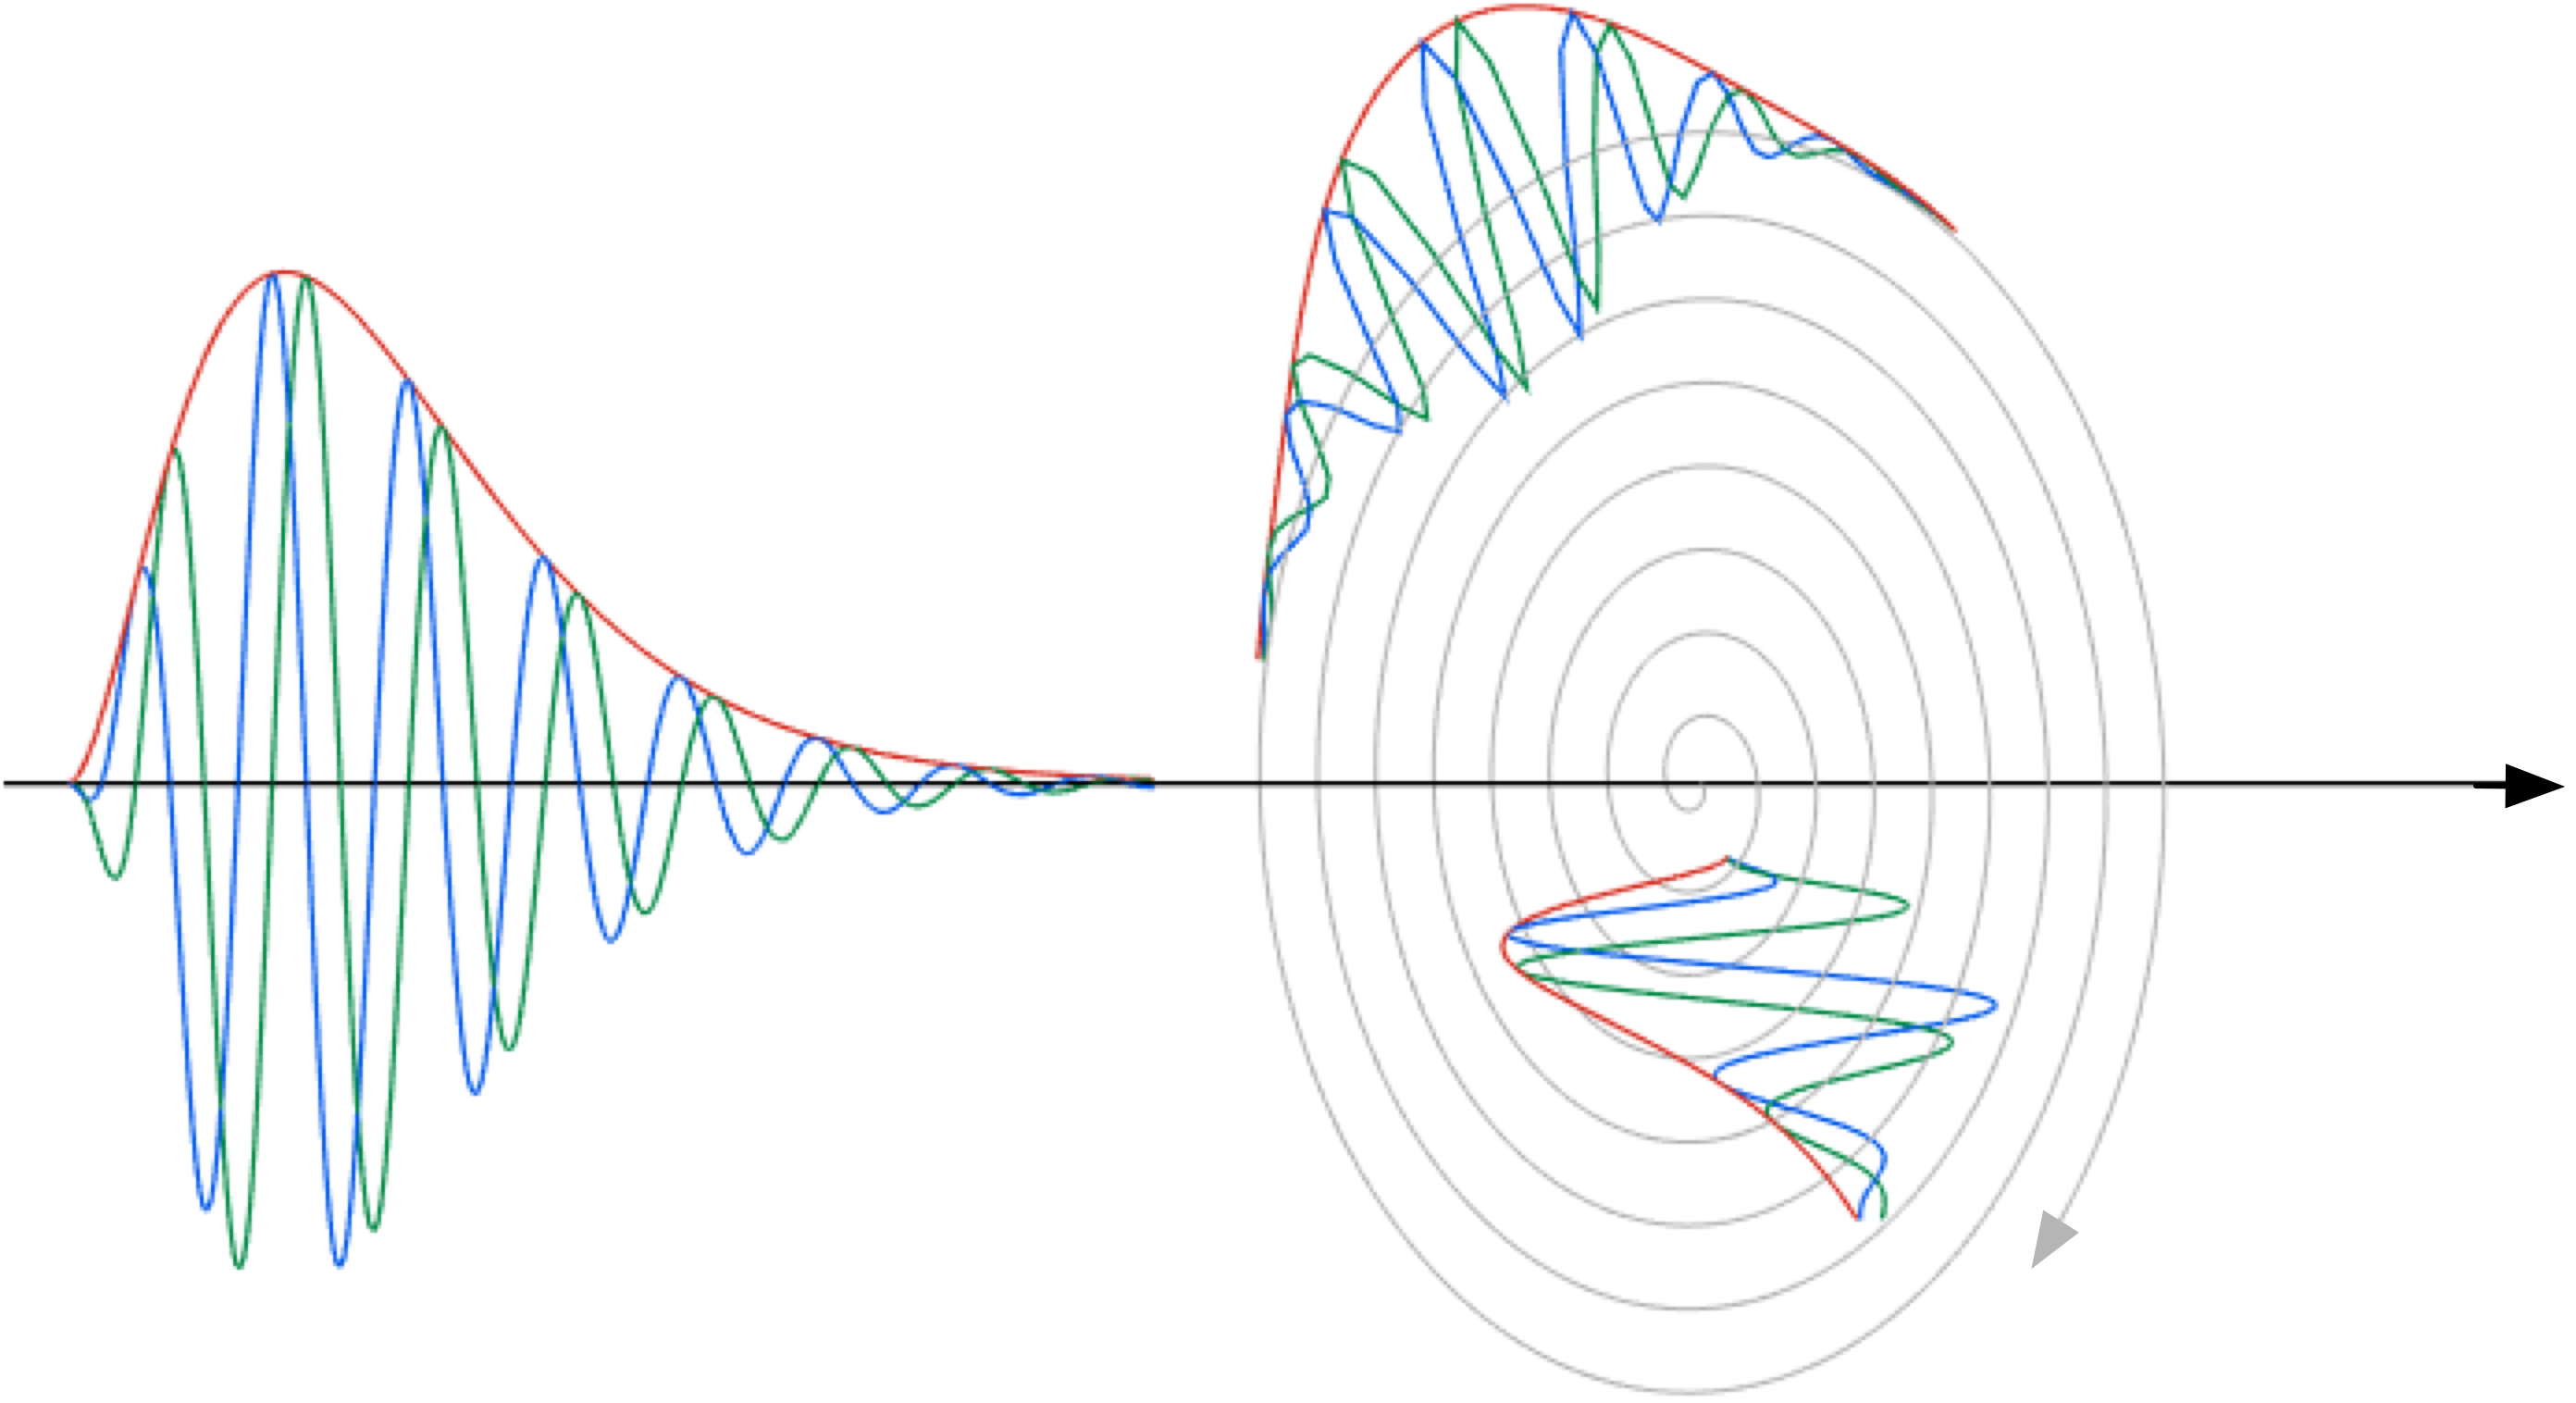
\includegraphics[width=8.5cm]{../figures/fig1/raw_fig1.png}}
		\end{picture}
	\end{center}
	\protect\caption{
\label{fig:spiral-wavelets}
}
\end{figure}


\section{Shepard spiral scattering}

Let $\psi(t)=\vert\psi\vert(t)\mathrm{e}^{2\pi\mathrm{i}t}$ a "mother wavelet" of dimensionless center frequency $1$ and bandwidth $Q^{-1}$.
The quality factor $Q$ is an integer in the typical range $12$\textendash$24$.
Center frequencies of the subsequent wavelet filter bank are of the
form $\lambda_{1} = 2^{j_{1} + \frac{\chi_{1}}{Q}}$, where the indices
$j_{1} \in \mathbb{Z}$ and $\chi_1 \in \{1\ldots\,Q\}$ respectively denote
octave and chroma. The Fourier transform $\widehat{\psi}(\omega)$ of $\psi(t)$ is dilated by resolutions $\lambda_1$ to obtain wavelets $\widehat{\psi_{\lambda_1}}$ in the frequency domain:

\[
\widehat{\psi_{\lambda_{1}}}(\omega)=\widehat{\psi}(\lambda^{-1}\omega)
\quad\mathrm{i.e.}\quad
\psi_{\lambda_{1}}(t)=\lambda_{1}\psi(\lambda_{1}t).
\]

The wavelet transform of an audio signal $x(t)$ is defined as the array of convolutions $x \ast \psi_{\lambda_1}(t)$ for every audible frequency $\lambda_1$. The modulus of the resulting signals, called \emph{scalogram}, localize the power spectrum of $x(t)$ around the log-frequencies $\log_2 \lambda_1 = j_1 + \frac{\chi_1}{Q}$ over durations $2 Q \lambda_1^{-1}$, trading frequency resolution for time resolution:

\[
x_1 (t, \log_{2}\lambda_{1}) = \left| x \ast \psi_{\lambda_{1}} \right| (t).
\]

The constant-Q transform (CQT) $S_1 x$ corresponds to a lowpass filtering of $x_1$ with a window $\phi(t)$ of size $T$.

\[
S_1 x (t, \log_2 \lambda_1) = x_1 \ast \phi_T (t) = \left| x \ast \psi_{\lambda_{1}} \right| \ast \phi_T (t).
\]

There is a well-known dilemma in choosing $T$. Too small, the constant-Q matrix lacks invariance to time shifts, which will prevent any learning step to generalize from $S_1 x$ ; too large, discriminative information is discarded.

In order to combine the best of both worlds, the scattering transform recovers finer time scales than $T$ with a second filterbank of wavelets $\psi_{\lambda_2}(t)$ of center frequencies $\lambda_2$, and applies complex modulus to improve regularity \cite{Anden2014DSS}. The wavelets $\psi_{\lambda_2}(t)$ have a quality factor in the range  $1$\textendash$2$, though we choose to keep the same notation $\psi$ for simplicity.

\[
x_2 (t, \log_2 \lambda_1, \log_2 \lambda_2) =
\left| \left| x \ast \psi_{\lambda_{1}} \right|  \ast \psi_{\lambda_{2}} \right| (t) 
\label{eq:time-scattering}
\]

Also known as \emph{amplitude modulation spectrum}, the three-way array $x_2$ is then averaged in time to achieve as much invariance as the constant-Q spectrum $S_1 x$:

\[
S_2 x (t, \log_2 \lambda_1, \log_2 \lambda_2) =
\left| \left| x \ast \psi_{\lambda_{1}} \right|  \ast \psi_{\lambda_{2}} \right| (t)  \ast \phi_T (t).
\]

The concatenated scattering representation $Sx = \{S_1 x, S_2 x \}$ has proven to achieve higher accuracy in music genre classification as well as phoneme recognition \cite{Anden2014DSS} than audio features derived from $S_1 x$ only, such as Mel-frequency cepstral coefficients (MFCC).

Due to the constant-Q property, $Sx$ is stable to small time warps of $x(t)$, as long as they do not exceed $Q^{-1}$, i.e. one semitone.
This implies that small modulations, such as tremolo and vibrato, are accurately linearized in rate and depth \cite{Anden2012}.

However, the definition above is unstable to the variability in pitch and spectral envelope, for which the activation of frequency bands is highly correlated in time.
To stabilize $x_2$ with respect to these variations, And�n \cite{Anden2014PhD} has redefined the wavelets $\psi_{\lambda_2}$'s as two-dimensional functions of both time and log-frequency, indexed by pairs $\lambda_2 = (\alpha,\beta)$, where $\alpha$ is measured in Hertz and $\beta$ is measured in cycles per octaves. 

\[
\psi_{\lambda_2}(t,\log_2 \lambda_1) = \psi_\alpha (t) \times \psi_\beta (\log_2 \lambda_1)
\]

The equation below introduces a "joint time-frequency scattering" transform, as opposed to the plain "time scattering" transform of Equation \ref{eq:time-scattering}.

--- DRAFT BELOW---


It should be noted that, while the definition above successfully describes the average spectral envelope and amplitude modulation of a signal, it decomposes and averages each frequency band separately. Hence, it cannot properly characterize the joint time-frequency structure of natural sounds.

\[
\log_2 \lambda_1 = \lfloor \log_2 \lambda_1 \rfloor + \{ \log_2 \lambda_1 \}
\]

\[
\Psi_{\lambda_2}(t, \log_2 \lambda_1) =
\psi_{\alpha}(t) \times
\psi_{\beta}(\log_2 \lambda_1) \times
\psi_{\gamma}(\lfloor \log_2 \lambda_1 \rfloor)
\]

The integer part $\lfloor \log_2 \lambda_1 \rfloor$ is the octave index (related to perceived pitch height), whereas the fractional part $\{ \log_2 \lambda_1 \}$ is related to pitch chroma.

\section{Deformations of the source-filter model}

\[
x(t) = \left[ e_{\theta}\ast h_{\zeta} (t) \right]
\]

\begin{figure}[t]
	\begin{center}
		\setlength{\unitlength}{1cm}
		\begin{picture}(6,5.0)
		\put(0,0){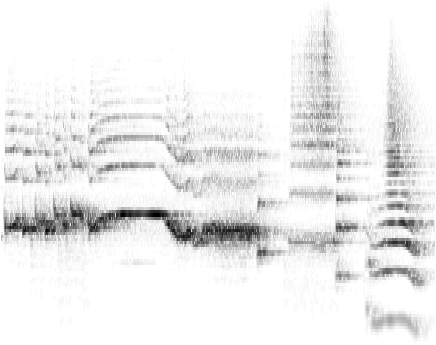
\includegraphics[width=6cm]{../figures/fig4/raw_fig4.png}}
		\end{picture}
	\end{center}
	\protect\caption{
\label{fig:berio-scalogram}
}
\end{figure}

%\[
%S_1 x(t,\log_2 \lambda_1) \propto
%\widehat{\psi_{\lambda_1}}\left( 2^{k(t,\log_2 \lambda_1) + LDLD[\theta](t)} f_0 \right) \times
%g\left(  \right)
%\]

\section{Conclusions}

The spiral model is well-known in music theory and experimental psychology. However, existing methods in audio signal processing do not fully take advantage from its richness, as they either picture pitch on a line (e.g. MFCC) or on a circle (e.g. chroma features).

Future work will be devoted to evaluating the discriminative power of Shepard spiral scattering coefficients over a variety of classification pipelines. Our representation also encompass automatic music transcription, perceptual similarity learning, and new audio transformations as potential applications.

%\newpage
\nocite{*}
\bibliographystyle{IEEEbib}
\bibliography{Lostanlen_DAFx15} % requires file DAFx15_tmpl.bib
 
\end{document}
